Discrete Wavelet Transform (DWT) on a signal $x[n] \: (0 \leq n < N)$ is essentially
passing the signal through a filter function, $f$, 
in a convolution operator.
%
This filter function is also called the \textit{kernel} of this DWT.
%
The results of this DWT are \textit{coefficients} of the signal.
%
The coefficients can be further categorized as two separate groups: 
one representing an approximation of the original signal,
namely \textit{scale coefficients};
and another one contains the detailed information to reconstruct
the original signal from the approximation, namely 
\textit{detail coefficients}.
%
Normally each of these two groups of coefficients has a size $\frac{N}{2}$.


DWTs can also be applied on the coefficients from previous DWTs.
%
When applying another round of DWT, transforms are applied on the two
groups of coefficients separately.
%
As a result, the original singal $x[n]$ is represented as 4 groups of 
coefficients; each has a size $\frac{N}{4}$.
%
This iteration finishes when each of the coefficient groups are small enough,
or the number of iterations reaches the maxinum value set by the user. 
%
%Since a singal is decomposed into multiple groups of coefficients,
%this process is also named a \textit{decomposition}.
%
%Similarly, the reverse calculation, which reconstructs the original signal 
%from the coefficients, is named \textit{reconstruction}.
%
Figure~\ref{fig:example1} illustrates an example of DWT on an 8-element signal.


\begin{figure}[p]
    \centering
    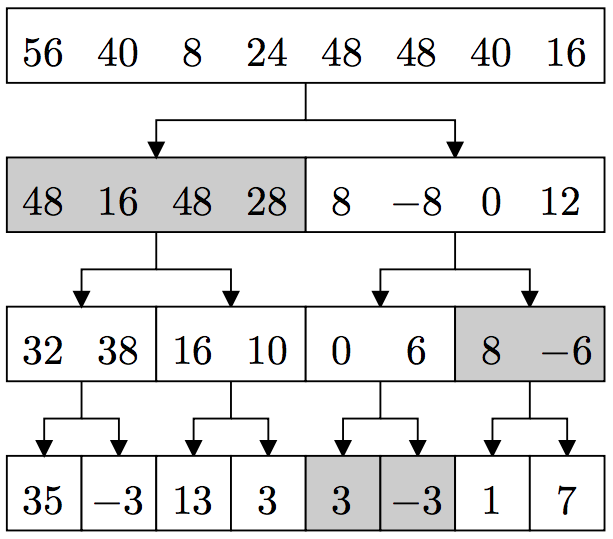
\includegraphics[width=0.8\textwidth]{fig/example1.png}
    \caption{An example of DWT on a signal with 8 elements.}
    \label{fig:example1}
\end{figure}






